\section{Kryptografi}
\begin{frame}
\frametitle{Innehåll}
\tableofcontents[currentsection]
\end{frame}

\begin{frame}{Kryptografi}

\begin{itemize}
\item Första 2000 år bc.
\item Public key crypto 1976
\end{itemize}


\begin{center}
  \makebox[0.8\textwidth]{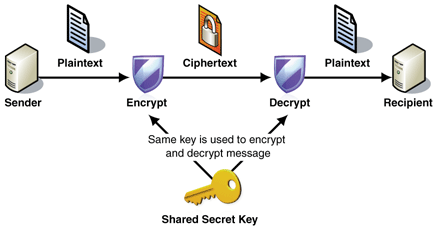
\includegraphics[width=0.8\textwidth]{images/symmetric.png}}
\end{center}

%% ¨ Oversiktlig beskrivning av kryptografi. Caesar-chiffer F¨orut fanns bara symmetriska, gemensam nyckel. xxxx bc. - 1976

\end{frame}

\begin{frame}{Public Key Cryptography}

%% En nyckel f¨or kryptering, en f¨or dekryptering

\begin{center}
  \makebox[0.8\textwidth]{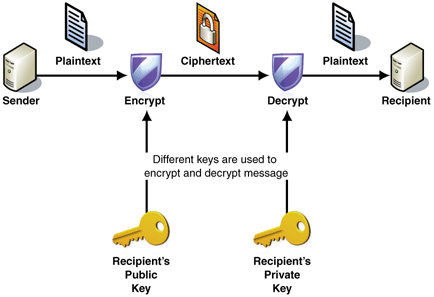
\includegraphics[width=0.8\textwidth]{images/asymmetric.png}}
\end{center}

\end{frame}

\begin{frame}

$$
y := g^x \mod{p}
$$

Givet y, g och p. Vad är x? Svårt! Tack vare detta så kan vi skapa El Gamal.

$$ y := g^{x} $$
$$ s random $$
$$ c = (g^s, y^s\cdot m) = (u, v) $$
$$ m = u^{-x}\cdot v = g^{-s\cdot x}\cdot y^s\cdot m = (g^x)^{-s}\cdot(g^x)^s\cdot m = m $$

Förklara hur lätt logaritm => knäckt krypto. Homomorfism, lager på lager Detta kan generaliseras till valfri cyklisk grupp.


\end{frame}

\begin{frame}{Zero-knowledge proof}

Bevisa att man besitter information utan att avslöja informationen. Exempel med sten, sax, påse genom kryptering. 

\end{frame}